%
% $Id: AttributeSet.java 15 2010-10-11 16:16:32Z justinkamerman $ 
%
% $LastChangedDate: 2010-10-11 13:16:32 -0300 (Mon, 11 Oct 2010) $ 
% 
% $LastChangedBy: justinkamerman $
%

\documentclass[10pt]{report}
\usepackage{graphicx}
\usepackage{setspace}			
\onehalfspacing

\title{CS6735 Programming Assignment 1}
\author{Justin Kamerman 3335272}
\date{\today}

\begin{document}
\maketitle
% No chapter numbers
\renewcommand*\thesection{\arabic{section}}

%----------------------------------------
% Assignment
%----------------------------------------
\section{Assignment}
\begin{enumerate} 
\item Implement ID3 algorithm using Java. Evaluate your implementation
  on the datasets in data.zip using 10 times 5-fold cross-validation,
  and report the average accuracy and standard deviation. All datasets
  are for UCI machine learning repository. You can check the detailed
  descriptions from the following link: 
  http://www.ics.uci.edu/~mlearn/MLRepository.html

For breast cancer data see:
http://archive.ics.uci.edu/ml/datasets/Breast+Cancer+Wisconsin+%28Diagnostic%29

For car data see:
http://archive.ics.uci.edu/ml/datasets/Car+Evaluation

For ecoli data see:http://archive.ics.uci.edu/ml/datasets/Ecoli

For letter recognition data see:
http://archive.ics.uci.edu/ml/datasets/Letter+Recognition

For mushroom data see: http://archive.ics.uci.edu/ml/datasets/Mushroom

\item Try to improve ID3 by some post pruning idea using a separate
  validation set.
\end{enumerate}

%----------------------------------------
% Learning Algorithm
%----------------------------------------
\section{Learning Algorithm}
\label{sec:learningalgorithm}
The program implements the ID3 decision tree building algorithm
described in \cite{Mitchell1997}. While the ID3 algorithm is
recursive, it has been implemented iteratively using an application
stack. This is a personal preference of the student based on past
experience with recursive programming causing JVM stack overflow
problems.

Initially, the decision trees constructed were unable to complete a
classification if the instance being classified encoded a path not
encountered in the training data i.e. no edge exists with value
matching instance attribute. To accomodate this scenario, when a new
attribute node is added to the tree, the most probable classification
within the training subset is stored in the node. During
classification, if no explicit edge exists matching an attribute  
value, the default classification is returned.

Missing attribute values are handled by preprocessing data sets,
replacing missing attribute value with the most probable value for the
attribute in the data set.

Attempt were made to counteract overfitting effects and improve the
accuracy of the ID3 decision trees using rule post-pruning
techniques. Various options were investigated but yielded very limited
benefits.

Initially, the original training set used by ID3 was reused for post
rule pruning. However the training set is biased towards the rule
chain and does not give accurate error estimates required for useful
pruning ~\cite{Frank2000}. This is consistent with our results, most
cases seeing a reduction in accuracy. Only one case,
ecoli.data, saw an improvement in accuracy but not to practical
levels of confidence.

Further pruning attempts were made using a separate pruning data set,
a technique called \textit{reduced-error pruning}. A portion of the training
data (25\% - 50\%) was held back for these purposes. Once again, all
but the ecoli.data saw reductions in accuracy, comparable to
the first pruning attempts. This technique had the disadvantage of
reducing the amount of training data available to ID3 for tree
construction ~\cite{Frank2000}.

From review of literature on the topic, it appears
that the success of decision tree pruning depends largely on the
ability to accurately estimate the error of a particular subtree or
rule. Based on error estimates, rules or nodes will be retained or
removed from the target hypothesis. The C4.5 decision tree algorithm,
a derivative of ID3, uses a statistical pessimistic error estimate
based on a selected confidence level. While only a heuristic and based
on some naive assumptions, this technique seems to work well in
practice ~\cite{Frank2000}. The student did not successfully implement
such a scheme to improve error estimates.


%----------------------------------------
% Data Sets
%----------------------------------------
\section{Data Sets}
Program expects data in CSV format with attributes occurring first and
classification at the end of each line. All data files have been
preprocessed to fit this format.


\subsection*{car.data}
\begin{itemize}
\item Number of Instances: 1728
\item Number of Attributes: 6
\item Attribute Values:
  \\\\
  \begin{left}
    \begin{tabular}{ l l }
      buying     & v-high, high, med, low \\
      maint      & v-high, high, med, low \\
      doors      & 2, 3, 4, 5-more \\
      persons    & 2, 4, more \\
      lug\_boot  & small, med, big \\
      safety     & low, med, high \\
    \end{tabular}
  \end{left}
  \\
\item Missing Attribute Values: none
\item Class Distribution (number of instances per class)
  \\\\
  \begin{left}
    \begin{tabular}{ l l }
      unacc   &  1210 \\
      acc     &   384 \\   
      good    &    69 \\     
      v-good  &    65 \\
    \end{tabular}
  \end{left}
\end{itemize}


\subsection*{ecoli.data}
\begin{itemize}
\item Number of Instances:  336
\item Number of Attributes: 7 
\item Attribute Values:
  \\\\
  \begin{left}
    \begin{tabular}{ l p{10cm} }
      mcg  &   McGeoch's method for signal sequence recognition. \\
      gvh  &   von Heijne's method for signal sequence recognition. \\
      lip  &   von Heijne's Signal Peptidase II consensus sequence score. Binary attribute. \\
      chg  &   Presence of charge on N-terminus of predicted lipoproteins. Binary attribute. \\
      aac  &   score of discriminant analysis of the amino acid content of outer membrane and periplasmic proteins. \\
      alm1 &   score of the ALOM membrane spanning region prediction program. \\
      alm2 &   score of ALOM program after excluding putative cleavable signal regions from the sequence. \\
    \end{tabular}
  \end{left}
  \\   
\item Missing Attribute Values: none.
\item Class Distribution (number of instances per class)
  \\\\
  \begin{left}
    \begin{tabular}{ l l }
      cp    &      143 \\
      im    &       77 \\               
      pp    &       52 \\
      imU   &       35 \\
      om    &       20 \\
      omL   &        5 \\
      imL   &        2 \\
      imS   &        2 \\
    \end{tabular}
  \end{left}
\end{itemize}


\subsection*{mushroom.data}
\begin{itemize}
\item Number of Instances: 8124
\item Number of Attributes: 22
\item Attribute Information:
  \\\\
  \begin{left}
    \begin{tabular}{ l p{10cm} }
      cap-shape                 &     bell=b, conical=c, convex=x, flat=f, knobbed=k, sunken=s \\
      cap-surface               &     fibrous=f, grooves=g, scaly=y, smooth=s \\
      cap-color                 &     brown=n, buff=b, cinnamon=c, gray=g, green=r, pink=p, purple=u, red=e, white=w, yellow=y \\
      bruises?                  &     bruises=t, no=f \\
      odor                      &     almond=a, anise=l, creosote=c, fishy=y, foul=f, musty=m, none=n, pungent=p, spicy=s \\
      gill-attachment           &     attached=a, descending=d, free=f, notched=n \\
      gill-spacing              &     close=c, crowded=w, distant=d \\
      gill-size                 &     broad=b, narrow=n \\
      gill-color                &     black=k, brown=n, buff=b, chocolate=h, gray=g, green=r, orange=o, pink=p, purple=u, red=e, white=w, yellow=y \\
      stalk-shape               &     enlarging=e, tapering=t \\
      stalk-root                &     bulbous=b, club=c, cup=u, equal=e, rhizomorphs=z, rooted=r, missing=? \\
      stalk-surface-above-ring  &     fibrous=f, scaly=y, silky=k, smooth=s \\
      stalk-surface-below-ring  &     fibrous=f, scaly=y, silky=k, smooth=s \\
      stalk-color-above-ring    &     brown=n, buff=b, cinnamon=c, gray=g, orange=o, pink=p, red=e, white=w, yellow=y \\
      stalk-color-below-ring    &     brown=n, buff=b, cinnamon=c, gray=g, orange=o, pink=p, red=e, white=w, yellow=y \\
      veil-type                 &     partial=p, universal=u \\
      veil-color                &     brown=n, orange=o, white=w, yellow=y \\
      ring-number               &     none=n, one=o, two=t \\
      ring-type                 &     cobwebby=c, evanescent=e, flaring=f, large=l, none=n, pendant=p, sheathing=s, zone=z \\
      spore-print-color         &     black=k, brown=n, buff=b, chocolate=h, green=r, orange=o, purple=u, white=w, yellow=y \\
      population                &     abundant=a, clustered=c, numerous=n, scattered=s, several=v, solitary=y \\
      habitat                   &     grasses=g, leaves=l, meadows=m, paths=p, urban=u, waste=w, woods=d \\
    \end{tabular}
  \end{left}

\item Missing Attribute Values: 2480, all for attribute #11.
\item Class Distribution: 
  \\\\
  \begin{left}
    \begin{tabular}{ l l }
      edible:     &  4208 (51.8\%) \\
      poisonous:  &  3916 (48.2\%) \\
      total:      &  8124 instances \\
    \end{tabular}
  \end{left}
\end{itemize}


\subsection*{letter-recognition.data}
\begin{itemize}
\item Number of Instances: 20000
\item Number of Attributes: 17 (Letter category and 16 numeric features)
\item Attribute Information:
  \\\\
  \begin{left}
    \begin{tabular}{ l p{10cm} }
      lettr	   &    capital letter	(26 values from A to Z) \\
      x-box	   &    horizontal position of box	(integer) \\
      y-box	   &    vertical position of box	(integer) \\
      width	   &    width of box			(integer) \\
      high 	   &    height of box			(integer) \\
      onpix	   &    total # on pixels		(integer) \\
      x-bar	   &    mean x of on pixels in box	(integer) \\
      y-bar	   &    mean y of on pixels in box	(integer) \\
      x2bar	   &    mean x variance			(integer) \\
      y2bar	   &    mean y variance			(integer) \\
      xybar	   &    mean x y correlation		(integer) \\
      x2ybr	   &    mean of x * x * y		(integer) \\
      xy2br	   &    mean of x * y * y		(integer) \\
      x-ege	   &    mean edge count left to right	(integer) \\
      xegvy	   &    correlation of x-ege with y	(integer) \\
      y-ege	   &    mean edge count bottom to top	(integer) \\
      yegvx	   &    correlation of y-ege with x	(integer) \\
    \end{tabular}
  \end{left}

\item Missing Attribute Values: None
\item Class Distribution:
  \\\\
  \begin{left}
    \begin{tabular}{ l l l l l l l }
 	789 A	   & 766 B     & 736 C     & 805 D	 & 768 E	   & 775 F     & 773 G \\
 	734 H	   & 755 I     & 747 J     & 739 K	 & 761 L	   & 792 M     & 783 N \\
 	753 O	   & 803 P     & 783 Q     & 758 R	 & 748 S	   & 796 T     & 813 U \\
 	764 V	   & 752 W     & 787 X     & 786 Y	 & 734 Z \\
    \end{tabular}
  \end{left}
\end{itemize}


\subsection*{breast-cancer.data}
\begin{itemize}
\item Number of Instances: 699
\item Number of Attributes: 10
\item Attribute Information: (class attribute has been moved to last column)
  \\\\
  \begin{left}
    \begin{tabular}{ l l }
      Clump Thickness               &  1 - 10  \\
      Uniformity of Cell Size       &  1 - 10  \\
      Uniformity of Cell Shape      &  1 - 10  \\
      Marginal Adhesion             &  1 - 10  \\
      Single Epithelial Cell Size   &  1 - 10  \\
      Bare Nuclei                   &  1 - 10  \\
      Bland Chromatin               &  1 - 10  \\
      Normal Nucleoli               &  1 - 10  \\
      Mitoses                       &  1 - 10  \\
    \end{tabular}
  \end{left}

\item Missing attribute values: 16
\item Class distribution: (2 for benign, 4 for malignant)
  \\\\
  \begin{left}
    \begin{tabular}{ l l }
      Benign       &  458 (65.5\%) \\
      Malignant    &  241 (34.5\%) \\
    \end{tabular}
  \end{left}
\end{itemize}


%----------------------------------------
% Program Design
%----------------------------------------
\section{Program Design}
The ID3 and rule post pruning algorithms are implemented by a Java
program. The only external dependency is on the Apache commons-cli
library for parsing commend line options. To that end, the program is
operated from the command line, taking options listed in table
~\ref{tab:commandline}.  
\\
\begin{table}[h]
  \centering
  \begin{tabular}{ |l|p{10cm}|} 
    \hline
    Option & Description \\ \hline
    -d          &  Generate Graphviz DOT output. \\ \hline
    -f \<arg\>  &  Path of data file \\ \hline
    -i \<arg\>  &  Number of iterations to perform. Default is 10 \\ \hline
    -n \<arg\>  &  A comma-separated list of attribute names, matching
    the order in which they appear in the data file \\ \hline
    -o \<arg\>  &  Number of folds to create in the training data during. Default is 5. \\ \hline
    -h          &  Print help message \\ \hline
  \end{tabular}
  \caption{Command line options}
  \label{tab:commandline}
\end{table}
\\\\
The program parses a data file, assumed to contain a set of training
instances on each line. Each training instance line is a
comma-separated list of attribute values terminated by a
classification or target value. Of the training data supplied for the
assignment, some had to be preprocessed to fit the expected format.

The program then executes a number of iterations (default is 10) over
the entire data set. During each iteration, the data set is folded
(default is 5 times), the training set used to create a decision
tree. The decision tree is then pruned. The details of the pruning
methodology are described in section ~\ref{sec:results}. The instances
in the test set are then evaluated by the decision tree and the pruned
rule set. The accuracy of the classifications is recorded for each
test set evaluated. After the final iteration is complete, the mean
accuracy and standard deviation are calculated and output by the
program.

The program implements various mechanism to facilitate
debugging. Throughout the code, log statements have been added using
the Java logging framework. The logging output is controlled for
individual classes via the \textit{logging.properties} file which the program
read on startup. In addition to logging, code was added to generate
Graphviz DOT (described in ~\cite{Graphviz2001}) output representing
the decision tree created. This output can be rendered using Graphviz
dot tool. An sample dot file for the mushroom.data data set is shown
below. The associated image generated by dot in Figure \ref{fig:dot}.


\begin{verbatim}
digraph G {
	23934262  [label="odor", shape=box];
	12617107  [label="p", shape=ellipse];
	23934262 -> 12617107 [label="y"];
	25277396  [label="p", shape=ellipse];
	23934262 -> 25277396 [label="m"];
	4536207  [label="e", shape=ellipse];
	23934262 -> 4536207 [label="l"];
	4368408  [label="spore-print-color", shape=box];
	23934262 -> 4368408 [label="n"];
	2741851  [label="e", shape=ellipse];
	4368408 -> 2741851 [label="y"];
	12064621  [label="e", shape=ellipse];
	4368408 -> 12064621 [label="h"];
	662907  [label="e", shape=ellipse];
	4368408 -> 662907 [label="k"];
	1409681  [label="e", shape=ellipse];
	4368408 -> 1409681 [label="o"];
	3087989  [label="e", shape=ellipse];
	4368408 -> 3087989 [label="n"];
	24688203  [label="p", shape=ellipse];
	4368408 -> 24688203 [label="r"];
	536608  [label="e", shape=ellipse];
	4368408 -> 536608 [label="b"];
	26188661  [label="habitat", shape=box];
	4368408 -> 26188661 [label="w"];
	19351067  [label="cap-color", shape=box];
	26188661 -> 19351067 [label="l"];
	23830114  [label="p", shape=ellipse];
	19351067 -> 23830114 [label="y"];
	7037649  [label="e", shape=ellipse];
	19351067 -> 7037649 [label="n"];
	2409492  [label="e", shape=ellipse];
	19351067 -> 2409492 [label="c"];
	29687596  [label="p", shape=ellipse];
	19351067 -> 29687596 [label="w"];
	5023414  [label="e", shape=ellipse];
	26188661 -> 5023414 [label="p"];
	5581355  [label="ring-number", shape=box];
	26188661 -> 5581355 [label="d"];
	21209219  [label="p", shape=ellipse];
	5581355 -> 21209219 [label="o"];
	14615126  [label="e", shape=ellipse];
	5581355 -> 14615126 [label="t"];
	17988434  [label="e", shape=ellipse];
	26188661 -> 17988434 [label="g"];
	6189088  [label="e", shape=ellipse];
	26188661 -> 6189088 [label="w"];
	1269167  [label="p", shape=ellipse];
	23934262 -> 1269167 [label="p"];
	23826509  [label="e", shape=ellipse];
	23934262 -> 23826509 [label="a"];
	13551501  [label="p", shape=ellipse];
	23934262 -> 13551501 [label="c"];
	26155569  [label="p", shape=ellipse];
	23934262 -> 26155569 [label="s"];
	50512  [label="p", shape=ellipse];
	23934262 -> 50512 [label="f"];
}
\end{verbatim}

\begin{figure}
  \begin{center}
	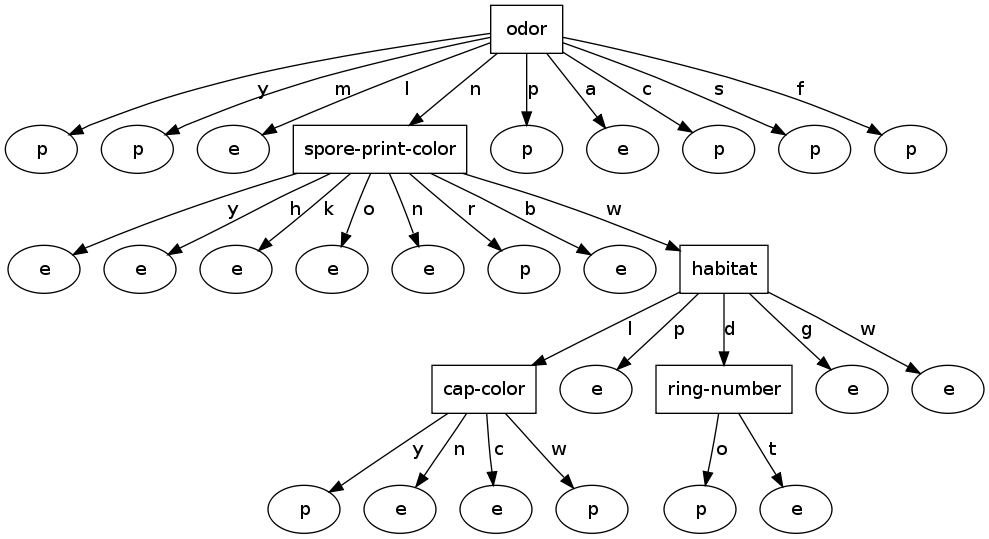
\includegraphics[angle=90,width=!,height=0.90\textheight]{mushroom}
  \end{center}
  \caption{Decision Tree visualization generated by DOT}
  \label{fig:dot}
\end{figure} 

\begin{figure}
  \begin{center}
	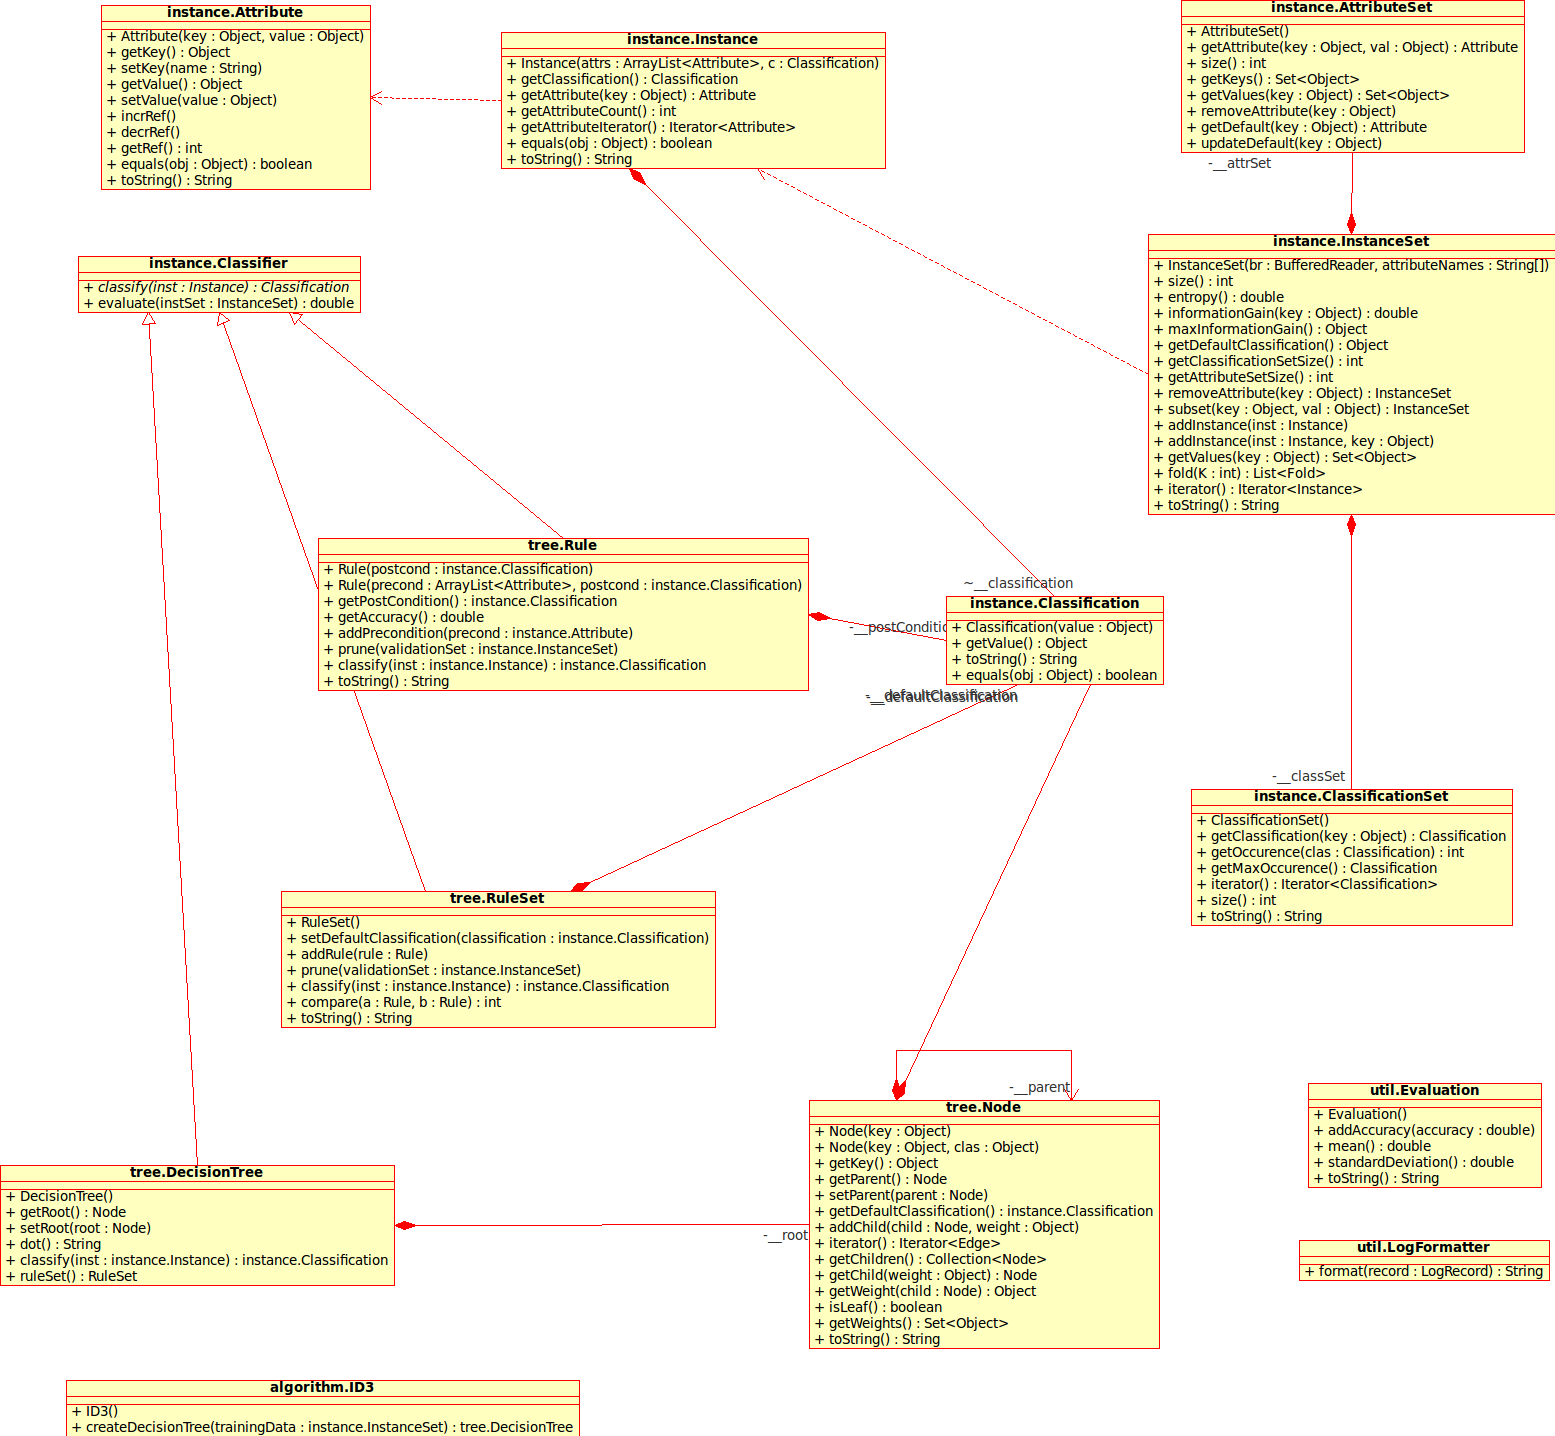
\includegraphics[angle=90,width=\textwidth,height=!]{uml}
  \end{center}
  \caption{UML class diagram}
  \label{fig:uml}
\end{figure} 

The implementation classes and their relationships are represented in a UML
class diagram in Figure \ref{fig:uml}. Following is a brief
description of each class:

\begin{itemize}
\item \textbf{Attribute} represents an attribute's name and value.

\item \textbf{AttributeSet} is a collection of attributes. It has
  convenience functions to determine attribute value range and
  probabilities of discrete values.

\item \textbf{Classification} represents an instance's classification
  or the value of the target function.

\item \textbf{ClassificationSet} is a collection of
  classifications. It has convenience functions to determine
  classification value range and probabilities of each
  classification. These functions are used extensively during the
  entropy calculation. 

\item \textbf{Classifier} is an interface implemented by any class
  which can take an instance and generate a classification for that
  instance. The interface is implemented by the \textit{DecisionTree},
  \textit{Rule}, and \textit{RuleSet} classes.

\item \textbf{DecisionTree} represents the decision tree constructed
  by the ID3 algorithm. It consists of a root node, representing the
  root of the decision tree, and a collection of functions to
  traverse the tree, prune the tree, generate dot output, generate a
  rule set and classify
  an instance. 

\item \textbf{Edge} represents an edge in the decision tree. Each Edge
  is associated with an attribute value.

\item \textbf{Evaluation} is a helper class for capturing test run
  accuracies and calculating final mean and standard deviation values.

\item \textbf{Fold} is an encapsulation of a training and a test set.
 
\item \textbf{ID3} implements the ID3 decision tree construction
  algorithm. It uses an application stack to model the recursive
  nature of the algorithm. This design choice was a preference of the
  student. While adding to the complexity of the implementation, the
  application stack has much larger capacity than the JVM stack. Stack
  capacity limits the recusive depth of the algorithm.

\item \textbf{Instance} represents a collection of attributes and
  their classification. In the case of training data, we use the
  classification to select the target hypothesis. In the case of test
  data, the classification is used to validate output of the target
  hypothesis.

\item \textbf{InstanceSet} is a collection of \textit{Instances}. This is the
  class that parses the data file and generates individual
  Instances. Functions exist to calculate entropy and information
  gain, create a subset of instance based on a particular attribute's
  value and fold the set of instances to create test and training sets
  of instances.

\item \textbf{LogFormatter} is a helper class to format log messages.

\item \textbf{Main} is the class which is started from the command
  line. It parses command line options and starts the test iterations.

\item \textbf{Node} represents a node in a decision tree. Each node is
  associated with either a particular attribute or classification
  depending on whether the node is an internal or leaf
  respectively. Internal nodes are associated with a default
  classification. This classification is the classification with the
  the highest probability in the instance subset associated with the
  subtree rooted at the given node. This default classification allows
  the decision tree to classify unseen instances even though an explicit
  path matching the instance's attribute values may not have been
  created during training. 

\item \textbf{Rule} represents a conjunctive classification rule with
  an arbitrary number of attribute preconditions and a classification
  postcondition. The classification interface will return the
  postcondition if a given instance's attributes matches the
  preconditions. Otherwise, null is returned indicating that the rule
  cannot classify the instance.

\item \textbf{RuleSet} is an ordered collection of rules. Rules are
  ordered by descending accuracy in approximating the target
  function. The RuleSet maintains a default classification, being the
  same as the default classification of the root node of the decision
  tree from whence it was generated i.e. the most probable
  classification in the original training set. The classification
  interface, given a test instance, will apply each of 
  its rules, in order, until one of them returns a non-null
  classification. If the end of the rule chain is reached before a
  classification is reached, the default classification of the rule
  set is returned.

\item \textbf{TreeIterator} is a helper class for performing a
  depth-first traversal of the decision tree.

\end{itemize}


%----------------------------------------
% Results
%----------------------------------------
\section{Results}
\label{sec:results}
The results of processing each data file through ten iterations of
5-fold cross-validation are presented below. The rule post-pruning
accuracy statistics were obtained using the training set for rule
pruning. As described in section \ref{sec:learningalgorithm}, this is
not a prescribed method for post pruning, however, the results were
not significantly different for other rule pruning techniques executed
so are included here for reference:

\subsection*{car.data}
{\small
\begin{verbatim}
[1:20:27][INFO][Main]: Loaded data from file data/car.data:
 [size=1728][entropy=1.205741][classificationSet=[[size=4][classifications=
[[[good][occurence=69]][[unacc][occurence=1210]][[acc][occurence=384]][[vgood]
[occurence=65]]]]]][attributes=[[doors][maint][safety][buying][lug_boot][persons]]]
 [1:20:27][INFO][Main]: Starting iteration 1 of 10
 [1:21:54][INFO][Main]: Starting iteration 2 of 10
 [1:23:19][INFO][Main]: Starting iteration 3 of 10
 [1:24:42][INFO][Main]: Starting iteration 4 of 10
 [1:26:07][INFO][Main]: Starting iteration 5 of 10
 [1:27:29][INFO][Main]: Starting iteration 6 of 10
 [1:28:54][INFO][Main]: Starting iteration 7 of 10
 [1:30:18][INFO][Main]: Starting iteration 8 of 10
 [1:31:42][INFO][Main]: Starting iteration 9 of 10
 [1:33:06][INFO][Main]: Starting iteration 10 of 10
 [1:34:30][INFO][Main]:

Test Results

ID3: [tests=50][mean accuracy=0.938377][standard deviation=0.015048]
Post-pruned: [tests=50][mean accuracy=0.722609][standard deviation=0.019412]
\end{verbatim}
}


\subsection*{ecoli.data}
{\small
\begin{verbatim}
[1:59:57][INFO][Main]: Loaded data from file data/ecoli.data:
[size=336][entropy=2.188746][classificationSet=[[size=8][classifications=
[[[imS][occurence=2]][[cp][occurence=143]][[imL][occurence=2]][[om][occurence=20]]
[[omL][occurence=5]][[pp][occurence=52]][[im][occurence=77]][[imU][occurence=35]]]]]]
[attributes=[[chg][aac][lip][gvh][alm1][mcg][alm2]]] 
[1:59:57][INFO][Main]: Starting iteration 1 of 10 
[2:00:03][INFO][Main]: Starting iteration 2 of 10 
[2:00:08][INFO][Main]: Starting iteration 3 of 10 
[2:00:14][INFO][Main]: Starting iteration 4 of 10 
[2:00:20][INFO][Main]: Starting iteration 5 of 10 
[2:00:25][INFO][Main]: Starting iteration 6 of 10 
[2:00:31][INFO][Main]: Starting iteration 7 of 10 
[2:00:36][INFO][Main]: Starting iteration 8 of 10 
[2:00:42][INFO][Main]: Starting iteration 9 of 10 
[2:00:48][INFO][Main]: Starting iteration 10 of 10 
[2:00:54][INFO][Main]: 

Test Results

ID3:		[tests=50][mean accuracy=0.384776][standard deviation=0.057519]
Post-pruned:	[tests=50][mean accuracy=0.432836][standard deviation=0.104691] 
\end{verbatim}
}


\subsection*{mushroom.data}
{\small
\begin{verbatim}
[2:51:56][INFO][Main]: Loaded data from file data/mushroom.data:
[size=8124][entropy=0.999068][classificationSet=[[size=2][classifications=
[[[e][occurence=4208]][[p][occurence=3916]]]]]][attributes=[[cap-surface]
[veil-color][odor][ring-number][gill-size][stalk-surface-below-ring][stalk-root]
[cap-shape][gill-color][stalk-surface-above-ring][gill-spacing][habitat]
[veil-type][cap-color][bruises?][stalk-color-above-ring][stalk-shape]
[stalk-color-below-ring][spore-print-color][gill-attachment][ring-type][population]]] 
[2:51:56][INFO][Main]: Starting iteration 1 of 10 
[3:00:32][INFO][Main]: Starting iteration 2 of 10 
[3:09:08][INFO][Main]: Starting iteration 3 of 10 
[3:17:47][INFO][Main]: Starting iteration 4 of 10  
[3:26:23][INFO][Main]: Starting iteration 5 of 10 
[3:35:02][INFO][Main]: Starting iteration 6 of 10 
[3:43:42][INFO][Main]: Starting iteration 7 of 10 
[3:52:22][INFO][Main]: Starting iteration 8 of 10 
[4:01:03][INFO][Main]: Starting iteration 9 of 10 
[4:09:42][INFO][Main]: Starting iteration 10 of 10 
[4:18:17][INFO][Main]: 

Test Results

ID3:		[tests=50][mean accuracy=1.000000][standard deviation=0.000000]
Post-pruned:	[tests=50][mean accuracy=0.538165][standard deviation=0.010261] 
\end{verbatim}
}


\subsection*{letter-recognition.data}
{\small
\begin{verbatim}
[5:44:54][INFO][Main]: Loaded data from file
data/letter-recognition.data:
[size=20000][entropy=4.699811][classificationSet=[[size=26][classifications=
[[[D][occurence=805]][[E][occurence=768]][[F][occurence=775]][[G][occurence=773]]
[[A][occurence=789]][[B][occurence=766]][[C][occurence=736]][[L][occurence=761]]
[[M][occurence=792]][[N][occurence=783]][[O][occurence=753]][[H][occurence=734]]
[[I][occurence=755]][[J][occurence=747]][[K][occurence=739]][[U][occurence=813]]
[[T][occurence=796]][[W][occurence=752]][[V][occurence=764]][[Q][occurence=783]]
[[P][occurence=803]][[S][occurence=748]][[R][occurence=758]][[Y][occurence=786]]
[[X][occurence=787]][[Z][occurence=734]]]]]][attributes=[[y-ege][xy2br][x-bar]
[x-ege][x2bar][x2ybr][width][xegvy][onpix][x-box][y2bar][y-bar][y-box][high][yegvx][xybar]]]  
[5:44:54][INFO][Main]: Starting iteration 1 of 10 
[10:23:27][INFO][Main]: Starting iteration 2 of 10 
[2:58:56][INFO][Main]: Starting iteration 3 of 10 
[7:33:33][INFO][Main]: Starting iteration 4 of 10 
[12:08:46][INFO][Main]: Starting iteration 5 of 10 
[4:45:24][INFO][Main]: Starting iteration 6 of 10 
[9:23:46][INFO][Main]: Starting iteration 7 of 10 
[2:08:24][INFO][Main]: Starting iteration 8 of 10 
[6:42:48][INFO][Main]: Starting iteration 9 of 10 
[11:17:12][INFO][Main]: Starting iteration 10 of 10 
[3:52:49][INFO][Main]: 

Test Results

ID3:		[tests=50][mean accuracy=0.760870][standard deviation=0.005610]
Post-pruned:	[tests=50][mean accuracy=0.101170][standard deviation=0.006650] 
\end{verbatim}
}


\subsection*{breast-cancer.data}
{\small
\begin{verbatim}
[2:36:30][INFO][Main]: Loaded data from file
data/breast-cancer-wisconsin.data:
[size=699][entropy=0.929318][classificationSet=[[size=2][classifications=
[[[2][occurence=458]][[4][occurence=241]]]]]][attributes=[[Uniformity_of_Cell_Size]
[Clump_Thickness][Bland_Chromatin][Uniformity_of_Cell_Shape][Marginal_Adhesion]
[Mitoses][Bare_Nuclei][Normal_Nucleoli][Single_Epithelial_Cell_Size]]] 
[2:36:30][INFO][Main]: Starting iteration 1 of 10 
[2:36:47][INFO][Main]: Starting iteration 2 of 10 
[2:37:03][INFO][Main]: Starting iteration 3 of 10  
[2:37:18][INFO][Main]: Starting iteration 4 of 10 
[2:37:35][INFO][Main]: Starting iteration 5 of 10 
[2:37:50][INFO][Main]: Starting iteration 6 of 10 
[2:38:06][INFO][Main]: Starting iteration 7 of 10  
[2:38:21][INFO][Main]: Starting iteration 8 of 10 
[2:38:36][INFO][Main]: Starting iteration 9 of 10 
[2:38:53][INFO][Main]: Starting iteration 10 of 10 
[2:39:09][INFO][Main]: 

Test Results

ID3:		[tests=50][mean accuracy=0.945899][standard deviation=0.017927]
Post-pruned:	[tests=50][mean accuracy=0.869928][standard deviation=0.031122] 

\end{verbatim}
}


%----------------------------------------
% Bibliography
%----------------------------------------
\bibliography{bibliography}
\bibliographystyle{plain}


%--------------------------------------------------
\end{document}
